\section{Zielsetzung}
In diesem Versuch wird das Geiger-Müller-Zählrohr auf seine Funktionen und Eigenschaften untersucht.
Hierzu wird die Charakteristik des Zählrohrs untersucht, sowie die freigesetzte Ladungsmenge und die Totzeit gemessen.


\section{Theoretische Grundlagen}
Mit dem Geiger-Müller-Zählrohr kann ionisierende Strahlung detektiert und dessen Intensität gemessen werden.
Sobald ionisierende Strahlung in das Zählrohr eintritt, wird ein Impuls abgegeben der mittels Impulszähler gezählt werden kann.

\subsection{Aufbau und Funktionsweise des Geiger-Müller-Zählrohrs}

\begin{figure}
            \centering
               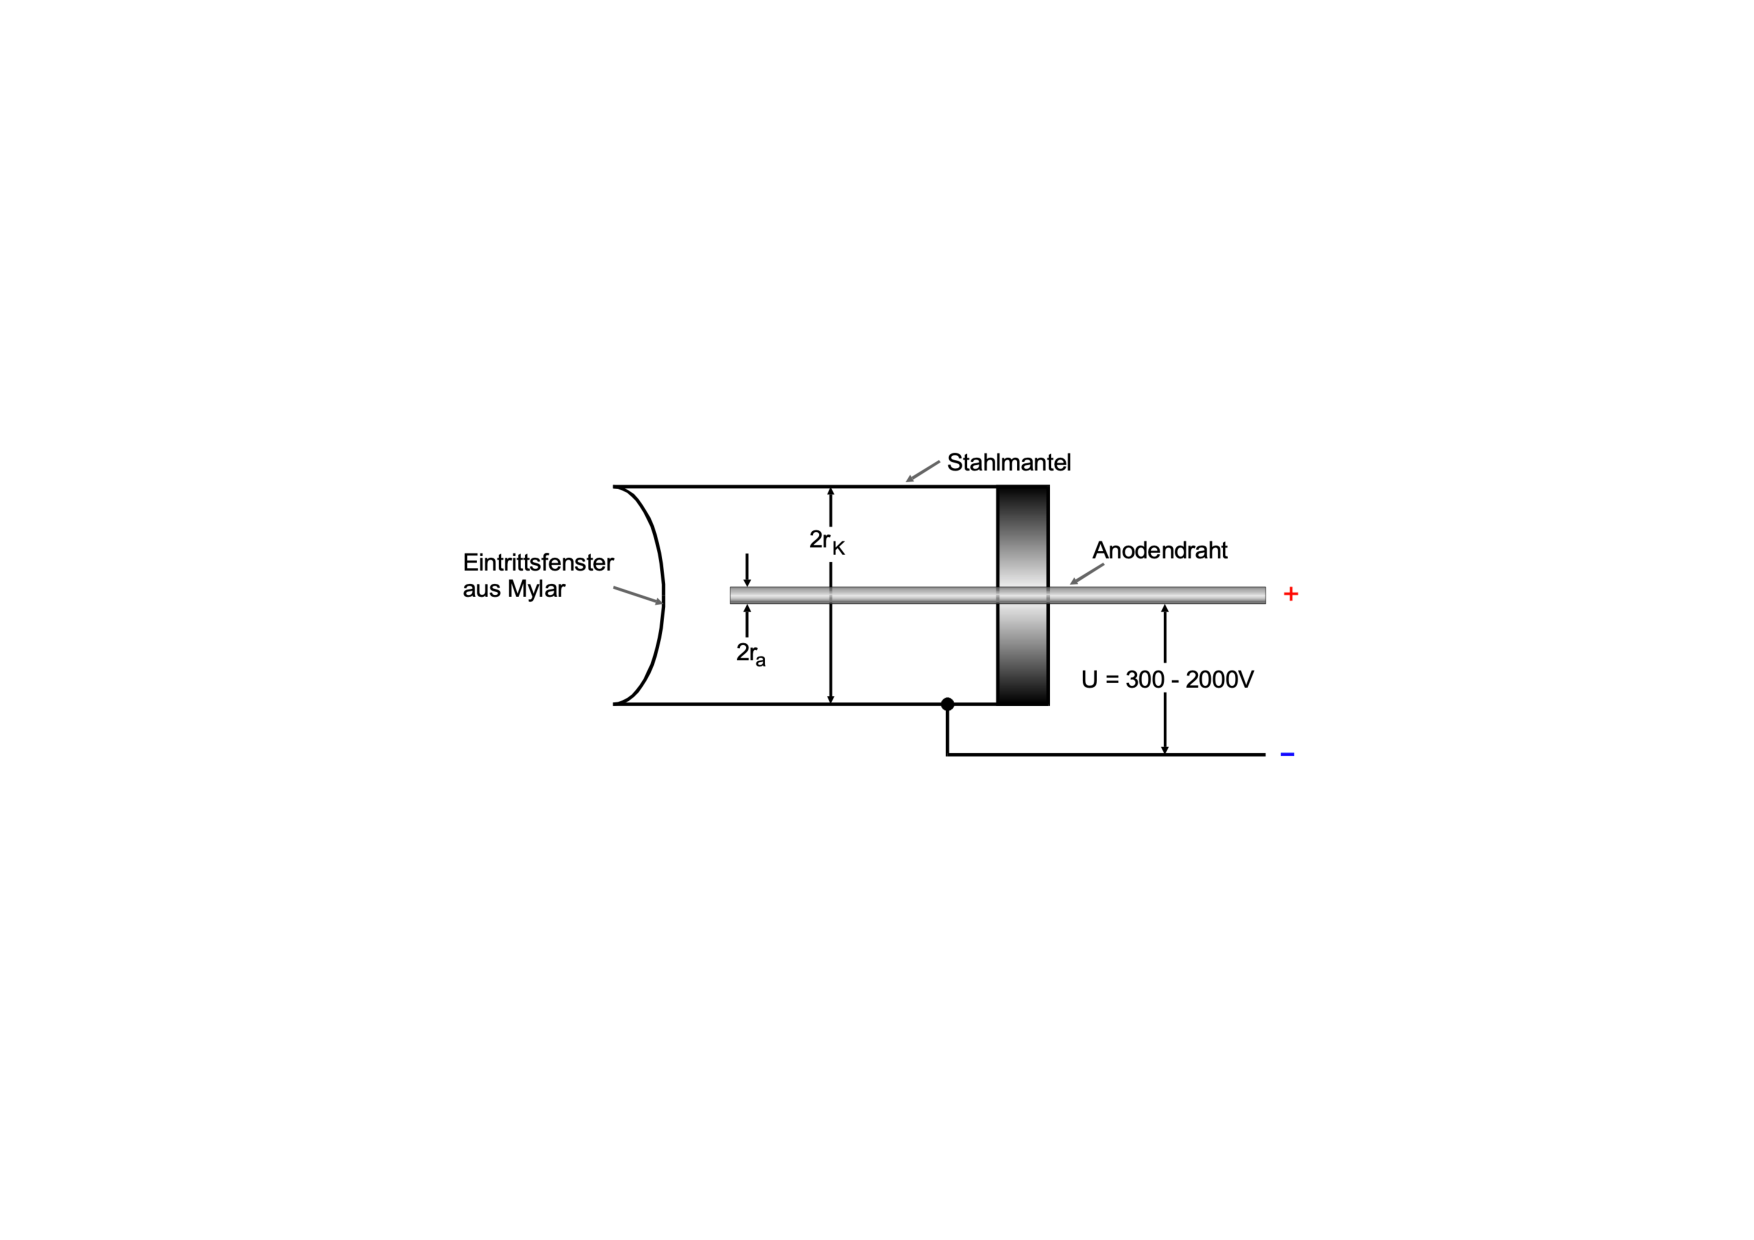
\includegraphics[height=5cm]{rohr.pdf}
               \caption{Aufbau eines Zählrohres (Quelle: \cite{V703}).}
               \label{fig:rohr}
        \end{figure}

\noindent
Das Zählrohr hat den in Abbildung (\ref{fig:rohr}) dargestellten Aufbau und besteht aus einer zylinderförmigen Kathode (Radius $\text{r}_\text{k}$), 
in der sich mittig, parallel zum Mantel, ein Anodendraht (Radius $\text{r}_\text{a}$) befindet.
An die Öffnung des Rohres, wo die ionisierende Strahlung eintreten soll, wird Mylar-Folie gespannt, die sich durch einen Unterdruck nach Innen wölbt.
Das Rohr ist mit einem Gasgemisch, wie zum Beispiel aus Argon und Ethylalkohol gefüllt.
Wird eine äußere Spannung angelegt, entsteht ein radialsymmetrisches Feld zwischen Kathode und Anode hat im Abstand r von der Zählrohrachse den Wert

\begin{equation}
\text{E}(\text{r}) = \frac{\text{U}}{\text{r} \, \text{ln}(\frac{\text{r}_\text{k}}{\text{r}_\text{a}})}.
\label{eqn:e}
\end{equation}

\noindent
Trifft ionisierende Strahlung in das Geiger-Müller-Zählrohr entstehen durch Ionisationsakte Elektronen und Ionen.
Die freien Elektronen werden durch das elektrische Feld (\ref{eqn:e}) zur Anode beschleunigt, wobei zwischen verschiedenen Spannungsgrößen unterschieden wird.

\newpage
\begin{figure}
            \centering
               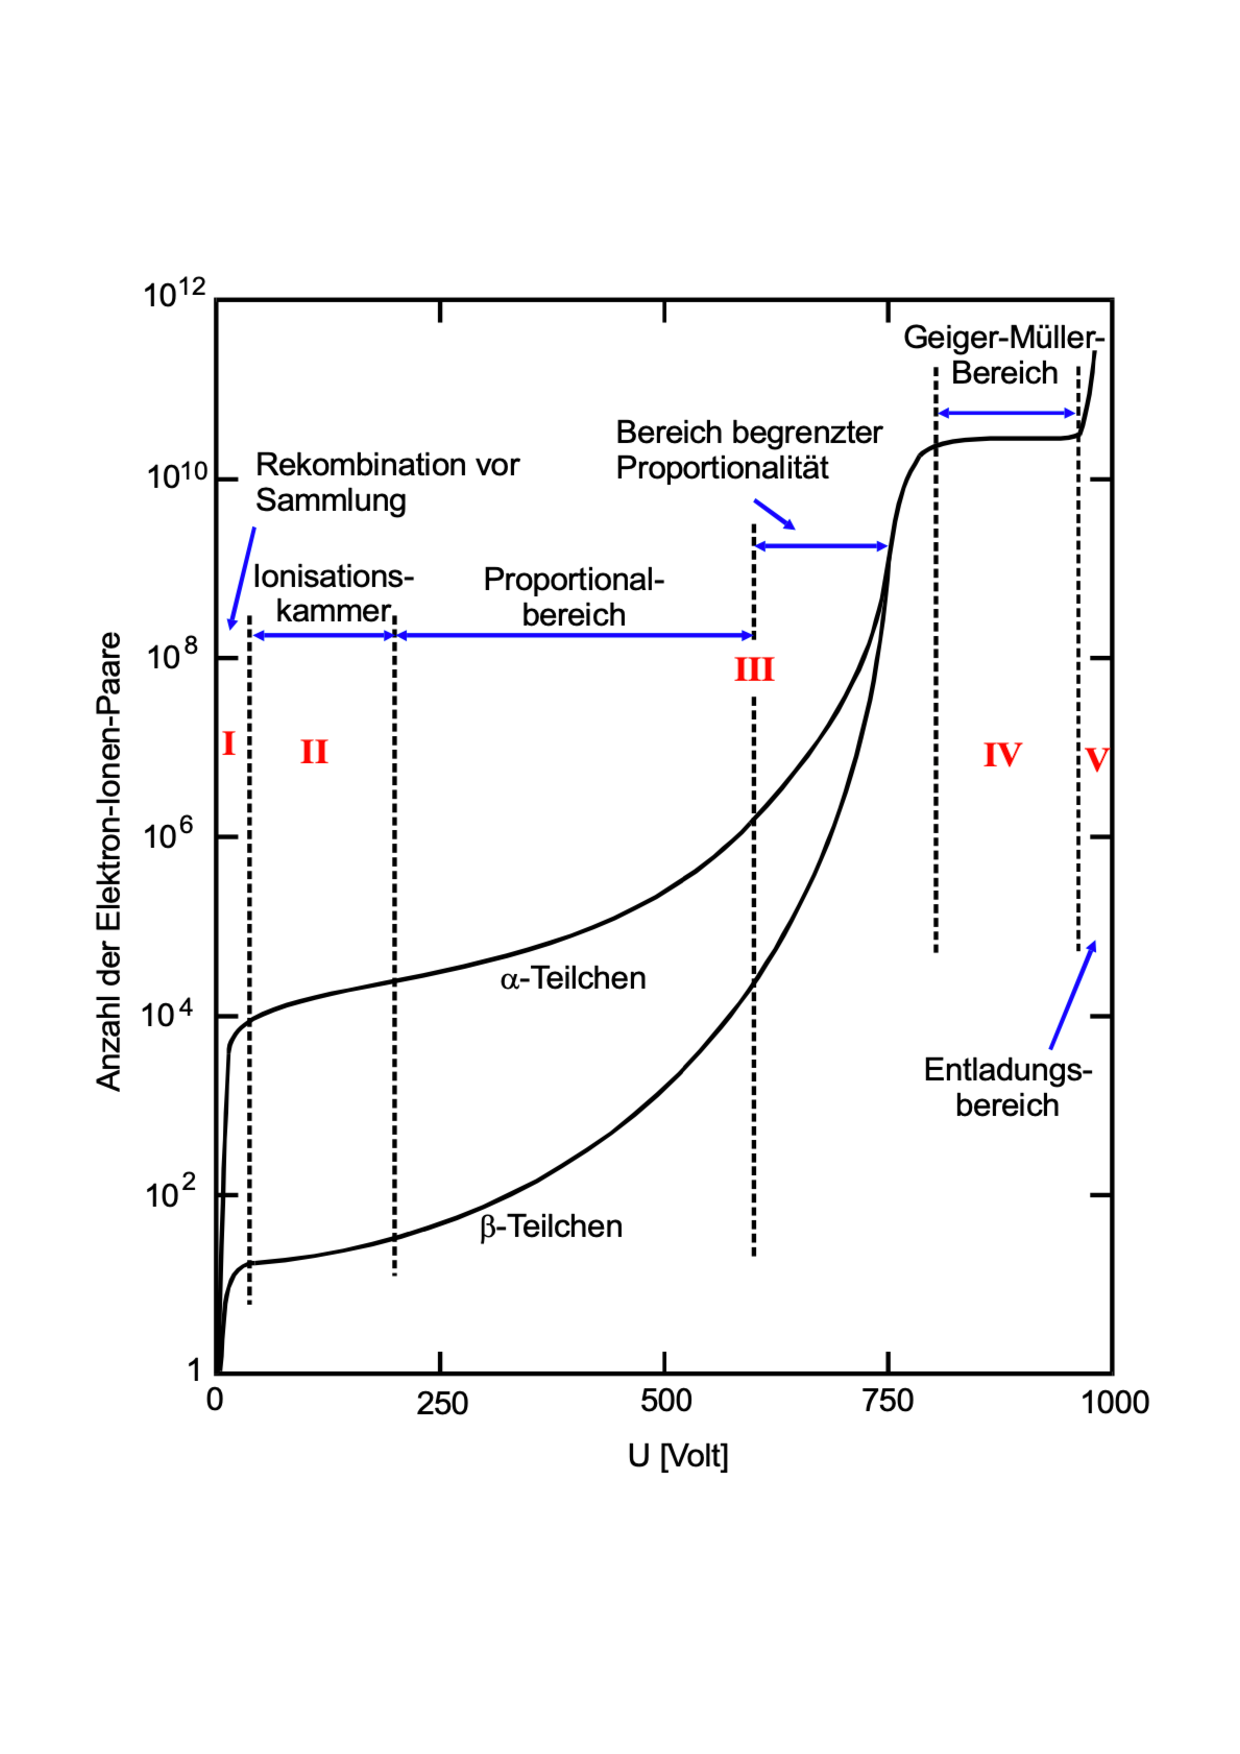
\includegraphics[height=12cm]{u.pdf}
               \caption{Anzahl der Elektron-Ionenpaare als Funktion der Spannung U (Quelle: \cite{V703}).}
               \label{fig:u}
        \end{figure}

\noindent
Im Folgenden werden die einzelnen Spannungsbereiche in Abbildung (\ref{fig:u}) näher erläutert.

\begin{enumerate}
\item Bei kleinen Zählrohrspannungen erreichen nicht alle Elektronen den Anodendraht und gehen durch Rekombination verloren.

\item Erhöht sich die Spannung und somit die Feldstärke, 
erreichen alle Elektronen den Draht und es fließt ein kontinuierlicher Ionisationsstrom der proportional zur Energie und Intensität der einfallenden Strahlung ist.
Eine solche Ionisationskammer kann aufgrund seiner geringen Ionisationsströme nur bei hohen Strahlungsintensitäten verwendet werden.

\item Bei weiterer Erhöhnung der Spannung werden die Elektronen so stark beschleunigt, dass es zur Stoßionisation kommt.
Die dadurch freigesetzten Elektronen können ebenfalls ionisieren, sodass es zu einer Townsend-Lawine kommt.
Die nun am Anodendraht gesammelte Ladung Q kann als Ladungsimpuls gemessen werden.
Da Q proportional zur Energie ist, die das einfallende Teilchen an das Gasvolumen abgegeben hat, 
ist der Ladungsimpuls ein Maß für die Teilchenenergie.
Aufgrund dieser Eigenschaft wird das Messinstrument als Proportionalzählrohr bezeichnet.

\item Wenn die Spannung über dem Propotionalitätsbereich liegt, wird der Auslösebereich erreicht, 
der eigentliche Arbeitsbereich des Geiger-Müller-Zählrohrs. 
Hier entsteht eine Großzahl an UV-Photonen, die sich im Gegensatz zu den Elektronen auch senkrecht zum elektrischen Feld ausbreiten können,
was zu Elektronenlawinen im gesamenten Zählrohrvolumen führt.
Bei so großer Spannung kann das Zählrohr effektiv nur als Intensitätsmesser eingesetzt werden. 

\item Ab einer noch größeren Spannung beginnt der Entladungsbereich.

\end{enumerate}

\subsection{Tot- und Erholungszeit}
Neben den Elektronen entstehen im Zählrohr positiv geladene Ionen, die durch ihre große Masse nur langsam zur Kathode beschleunigt werden.
In dieser Zeit baut sich eine radialsymmetrische Raumladung (Ionenschlauch) auf.
Dadurch wird die Feldstärke für eine Zeit T in Drahtnähe so gering, dass keine Stoßionisation mehr stattfindet und eintreffende Teilchen nicht registriert werden.
Diese Zeit T wird deswegen Totzeit genannt.
Wenn die positive Ladungswolke zur Kathode abwandert und die Feldstärke ansteigt, können eintreffende Teilchen wieder registriert werden.
Anschließend an die Totzeit T gibt es den Zeitraum der Erholungszeit $\text{T}_\text{E}$ , in dem die Ausgangsimpulse eine geringere Höhe haben.
Der Verlauf der Tot- und Erholungszeit ist in Abbildung (\ref{fig:totzeit})

\begin{figure}
            \centering
               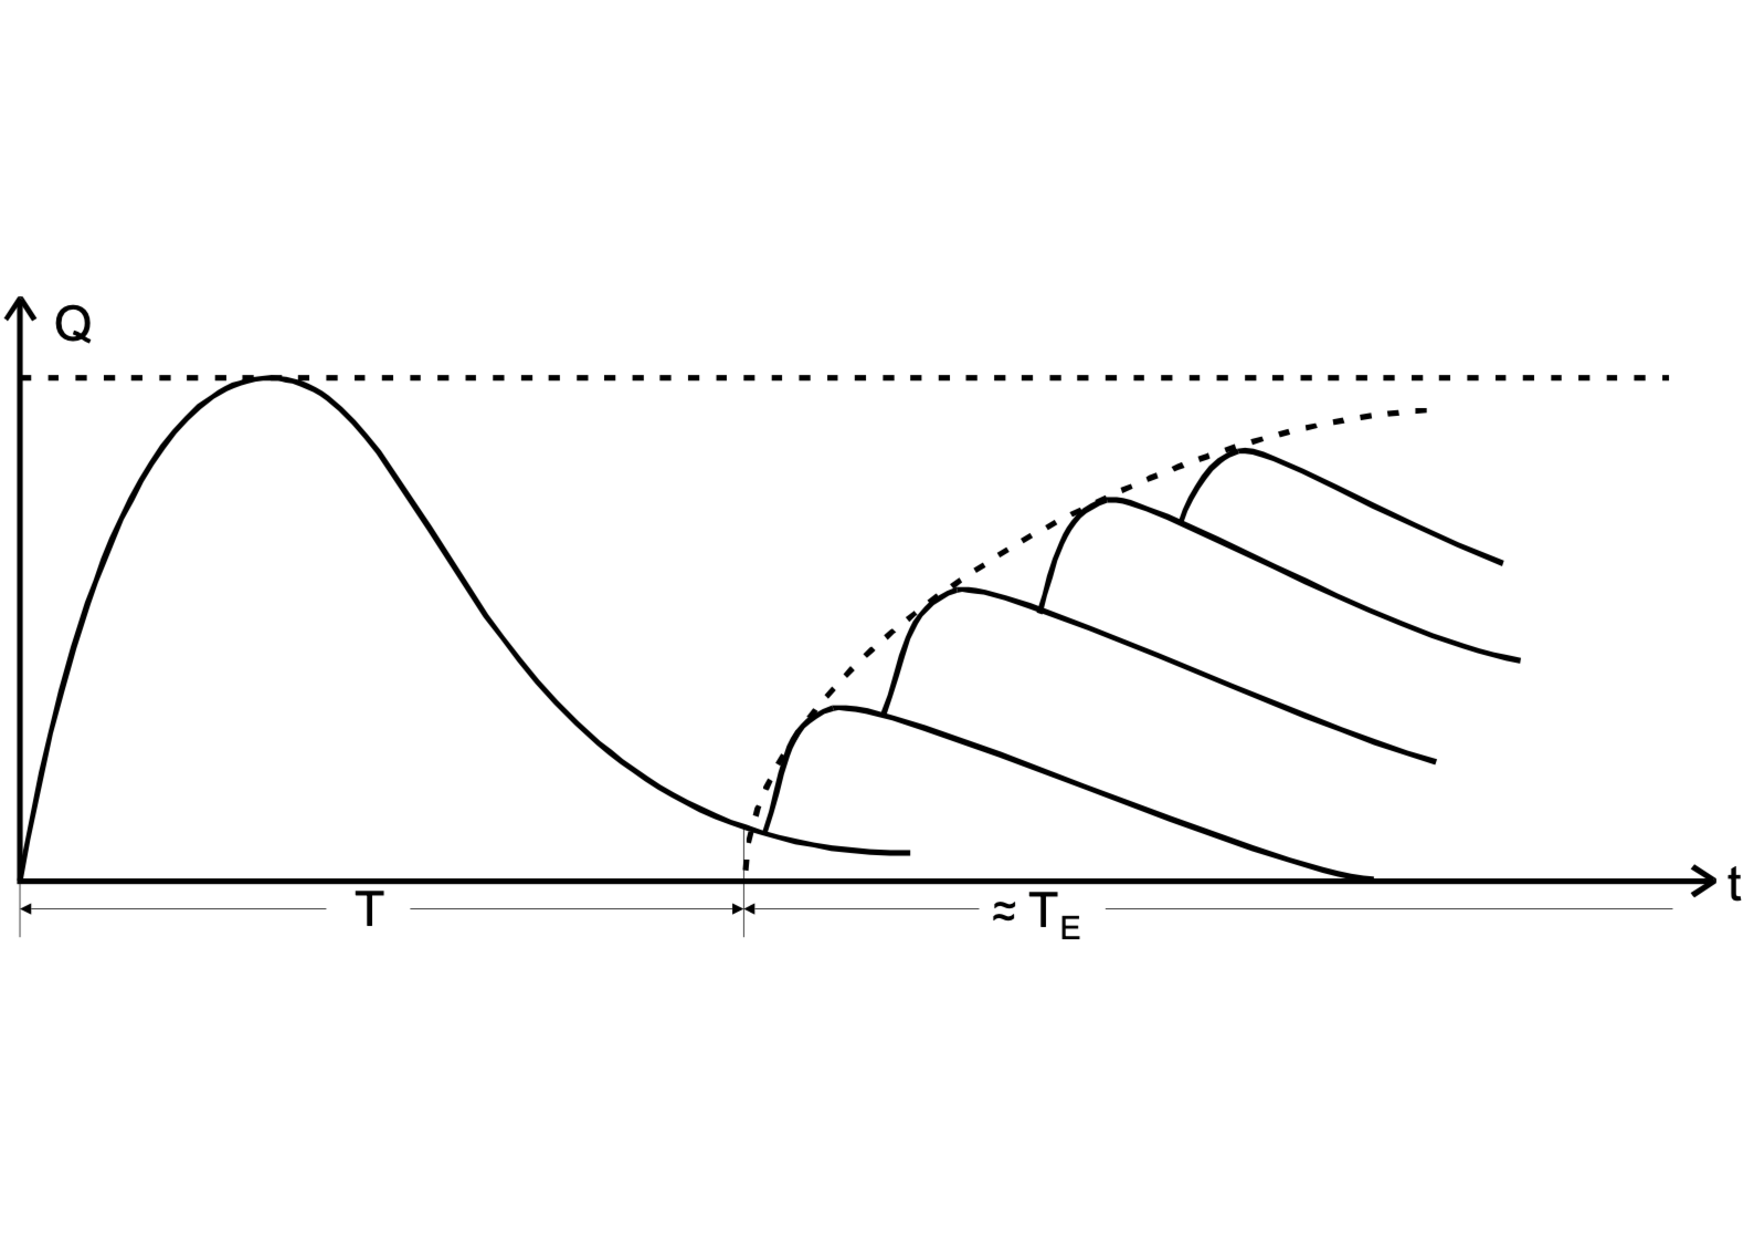
\includegraphics[height=5cm]{totzeit.pdf}
               \caption{Tot- und Erholungszeit eines Zählrohrs (Quelle: \cite{V703}).}
               \label{fig:totzeit}
        \end{figure}

\noindent
Wenn die Ionen auf die Zylinderkathode treffen, setzen sie bei der Neutralisation Elektronen aus der Metalloberfläche frei.
Diese Sekundärelektronen rufen weitere Zählrohrentladungen hervor, da sie das gesamte Zählrohrpotential U durchlaufen.
Der Durchgang eines Teilchens durch das Gasvolumen hat mehrere, zeitlich versetzte Ausgangsimpulse zur Folge, die als Nachentladungen bezeichnet werden.
Um die Nachentladung zu verhindern, wird dem Zählrohrgas Alkoholdampf hinzugefügt, damit bei der Neutralisation keine Elektronen freigesetzt werden.   

\newpage
\begin{figure}
            \centering
               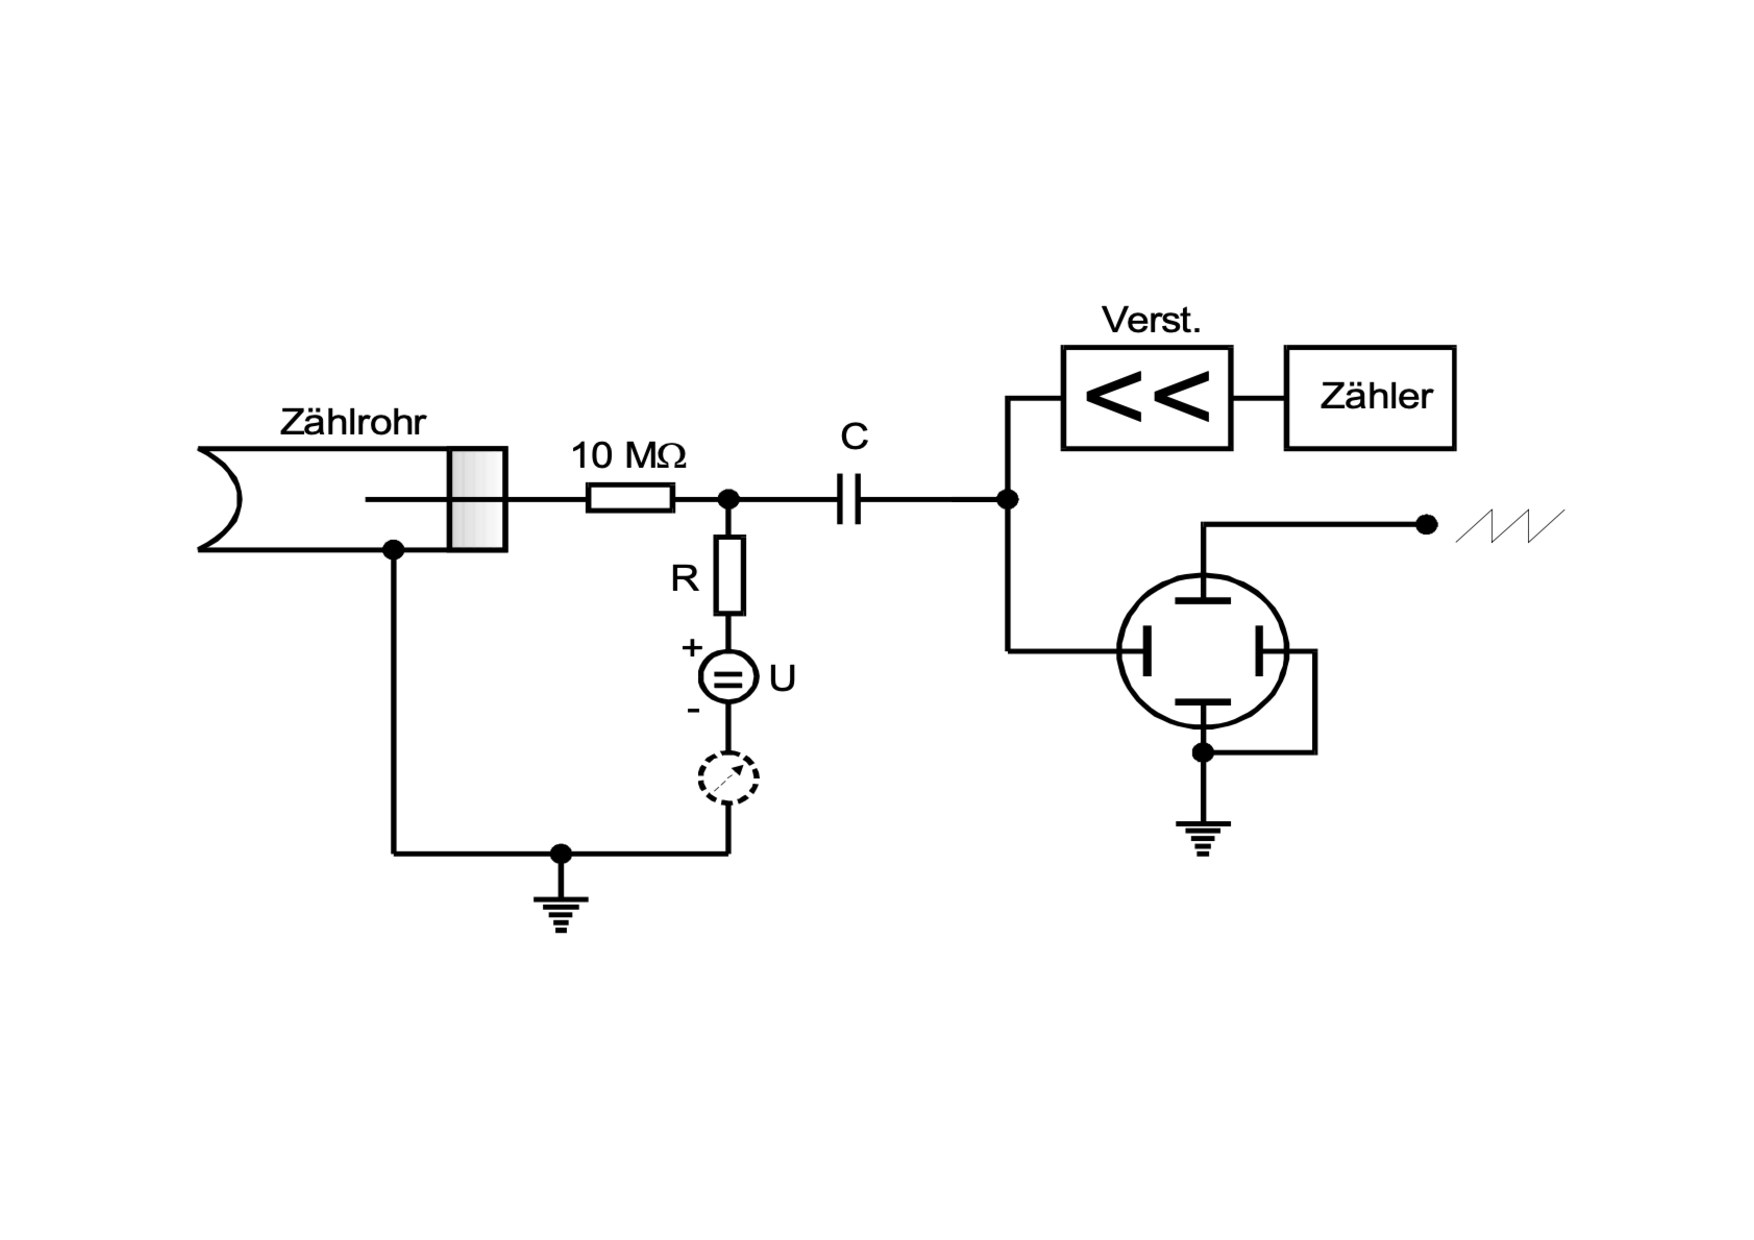
\includegraphics[height=5cm]{aufbau.pdf}
               \caption{Versuchsaufbau (Quelle: \cite{V703}).}
               \label{fig:aufbau}
        \end{figure}

\noindent
Die nachfolgenden Zählrohruntersuchungen können mit einem Versuchsaufbau nach Abbildung (\ref{fig:aufbau}) durchgeführt werden.
Sobald die Ladung Q auf dem Zähldraht über den Widerstand R abfließt wird ein Spannungsimpuls erzeugt, 
der über den Kondensator C ausgekoppelt, im Verstärker vergrößert und im Zählgerat registriert wird.

\noindent
Die Totzeit kann auf 2 verschiedene Arten bestimmt werden.
Die Oszillographische Messung ist eine Methode, bei der die Totzeit einem Oszillogramm gemäß Abbildung (\ref{fig:totzeit}) abgelesen werden kann.
Dabei sollte eine hohe Strahlungsintensität in das Zählrohr eintreten, 
wobei die Zeitablenkung des Oszillographen durch die Anstiegsflanke der Zählrohrimpulse getriggert wird.

\noindent
Das andere Messverfahren ist die Zwei-Quellen-Methode.
Durch die Totzeit T ist die registrierte Impulsrate $\text{N}_\text{r}$ immer kleiner als die Zahl $\text{N}_\text{w}$ der in das Zählrohr eingetretenen und absorbierten Teilchen.
Für die tatsächliche Impulsrate $\text{N}_\text{w}$ gilt:

\begin{equation}
\text{N}_\text{w}=\frac{\text{N}_\text{r}}{1-\text{T}\text{N}_\text{r}}.
\label{eqn:nw}
\end{equation}

\noindent
Um die Totzeit zu bestimmen, werden mit zwei radioaktiven Präparaten gemessen.
Zunächst wird die Zählrate $\text{N}_1$ des ersten Präparats gemessen.
Anschließend wird ein zweites Präparat daneben gestellt, sodass die beiden Präparate im gleichen Abstand zum Zählrohr stehen, 
ohne die Lage des ersten Präparats relativ zum Zählrohr zu verändern.
Diese Summenzählrate entspricht $\text{N}_{1+2}$.
Danach wird das erste Präparat entfernt und die Zählrate $\text{N}_2$ des zweiten Präparats wird registriert.

\noindent
Nach Gleichung (\ref{eqn:nw}) gilt:

\begin{equation*}
\text{N}_{\text{w}_1}=\frac{\text{N}_1}{1-\text{T}\text{N}_1}
\end{equation*}

\begin{equation*}
\text{N}_{\text{w}_2}=\frac{\text{N}_2}{1-\text{T}\text{N}_2}
\end{equation*}

\begin{equation*}
\text{N}_{\text{w}_{1+2}}=\frac{\text{N}_{1+2}}{1-\text{T}\text{N}_{1+2}}
\end{equation*}

\noindent
Da außerdem $\text{N}_{\text{w}_{1+2}}=\text{N}_{\text{w}_1}+\text{N}_{\text{w}_2}$ gilt, folgt

\begin{equation}
\frac{\text{N}_{1+2}}{1-\text{T}\text{N}_{1+2}}=\text{N}_{\text{w}_1}=\frac{\text{N}_1}{1-\text{T}\text{N}_1}+\text{N}_{\text{w}_2}=\frac{\text{N}_2}{1-\text{T}\text{N}_2}.
\label{eqn:nw12}
\end{equation}

\noindent
Gleichung (\ref{eqn:nw12}) lässt sich näherungsweise umschreiben zu

\begin{equation}
\text{T} \approx \frac{\text{N}_1 + \text{N}_2 - \text{N}_{1+2}}{2\text{N}_1\text{N}_2}.
\label{eqn:t}
\end{equation}


\subsection{Charakteristik des Zählrohres}
Die Charakteristik eines Zählrohres kann untersucht werden, 
indem die registrierte Teilchenzahl N bei konstanter Strahlungsintensität gegen die angelegte Spannung U aufgetragen wird.
Eine Charakteristik hat eine wie in Abbildung (\ref{fig:char}) gezeigte Gestalt.

\begin{figure}
            \centering
               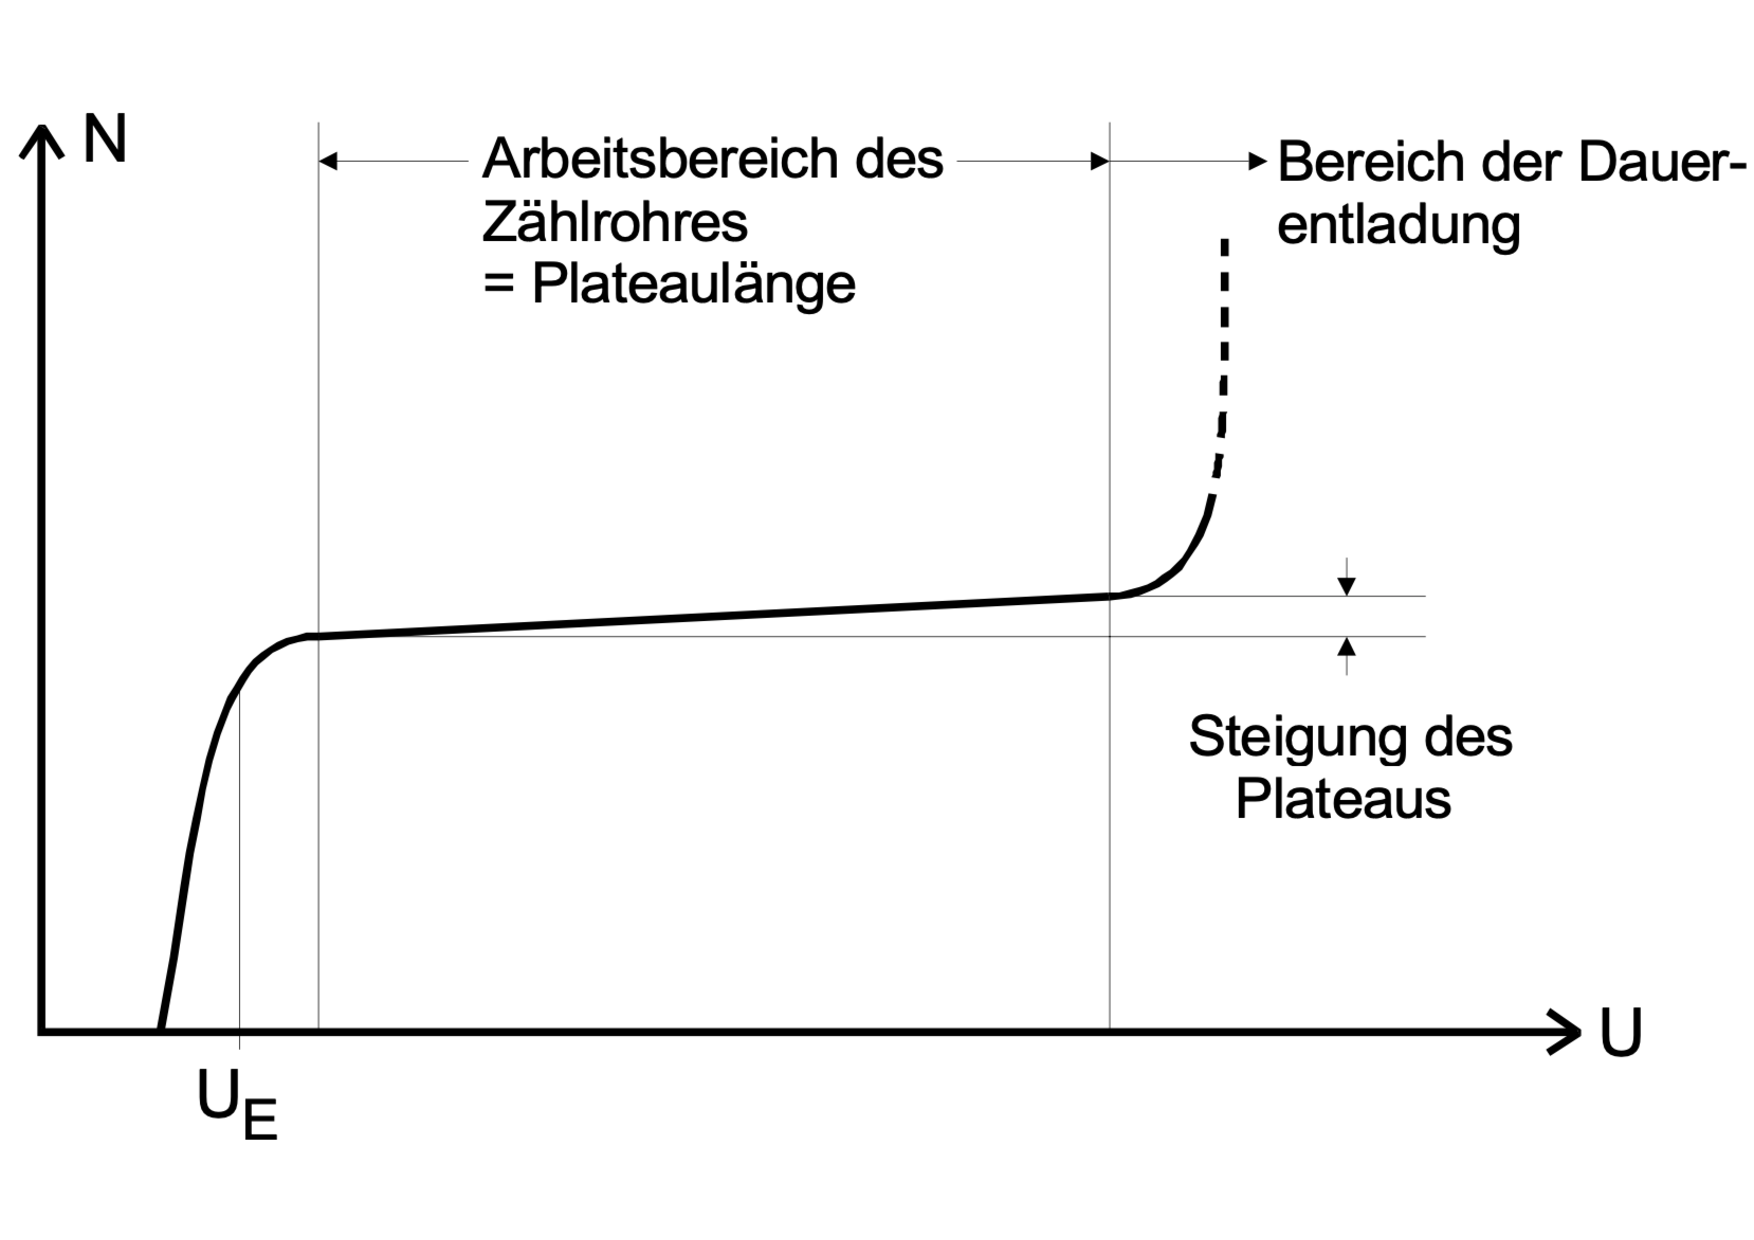
\includegraphics[height=7cm]{char.pdf}
               \caption{Charakteristik eines Zählrohres (Quelle: \cite{V703}).}
               \label{fig:char}
        \end{figure}

\noindent
Der lineare Teil der Kurve ist das Plateau, was eine Aussage über die Qualität des Zählrohres trifft.
Im Idealfall ist die Steigung des Plateaus gleich Null.
In der Praxis jedoch nimmt die Zählrate mit der Spannung aufgrung von einigen wenigen Nachentladungen zu.

\subsection{Ansprechvermögen des Zählrohres}
Das Ansprechvermögen ist die Wahrscheinlichkeit dafür, dass ein einfallendes ionisierendes Teilchen detektiert wird.
Für $\alpha$- und $\beta$-Teilchen liegt diese aufgrund ihres hohen Ionisationsvermögens nahezu bei 100$\%$.
Um sicher zu stellen, dass die Teilchen überhaupt in das Zählrohr eintreten, werden Endfensterzählrohre gebaut.
Diese haben eine Stirnseite aus einem dünnwandigen Material mit Atomen niedriger Ordnungszahl (hier Mylar), 
sodass auch $\alpha$-Teilchen sie durchdringen können.

\subsection{Die pro Teilchen vom Zählrohr freigesetzte Ladungsmenge}
Der mittlere Zählrohrstrom 

\begin{equation*}
\bar{\text{I}}=\frac{1}{\tau} \int_0^\tau \frac{\text{U}(\text{t})}{\text{R}} \, \text{dt}
\end{equation*}


\noindent
kann nach Abbildung (\ref{fig:aufbau}) gemessen werden.
Wenn die Impulszahl pro Zeiteinheit bekannt ist, kann daraus die pro Teilchen vom Zählrohr freigesetzte Ladungsmenge bestimmt werden.
Nach der Definition des Stromes gilt

\begin{equation}
\bar{\text{I}}=\frac{\Delta\text{Q}}{\Delta\text{t}}\text{Z}.
\label{eqn:i}
\end{equation}